% !TEX root = paper.tex
% \section{Proofs of Theorems}\label{app:proofs}

\section{Experimental Details}\label{app:setup}

\subsection{Model Configurations}\label{app:setup:model_configurations}
\textbf{FLUX.1-dev.}~\cite{flux2024}
We align the evaluation setup across compared acceleration methods
under the same sampling and hardware configuration.

\textbf{HiDream-I1-full.}~\cite{hidreami1technicalreport}
We align the evaluation setup across compared acceleration methods
under the same sampling and hardware configuration.

\textbf{Wan2.1.}~\cite{wan2025}
We align the evaluation setup across compared acceleration methods
under the same sampling and hardware configuration.

\textbf{HunyuanVideo.}~\cite{kong2024hunyuanvideo}
We align the evaluation setup across compared acceleration methods
under the same sampling and hardware configuration.
Note that due to TaylorSeer's memory requirements exceeding a single H800 GPU capacity,
we evaluate it on four H20 GPUs at the official resolution of $832\times640$
as specified in the official configuration.

\section{%
    Additional Experimental Results and Discussions
}\label{app:results}

\subsection{Wan2.1 VBench Results}\label{app:results:wan21-vbench}
We report additional Wan2.1 results
using VBench scores,
including a sweep over the cache history length $\mathcal{H}$
and the maximum number of consecutive cached steps $\mathcal{S}_{\max}$.
We report both efficiency metrics
(latency and speedup)
and the per-dimension VBench breakdown.
We report results across all evaluated configurations
in \Cref{tab:app:wan21-vbench-8dims}.
\begin{table}[t]
\centering
\caption{Wan2.1 VBench results for $\mathrm{D}^3$-Cache across cache hyperparameters (speedup is relative to the baseline).}
\label{tab:app:wan21-vbench-8dims}
\adjustbox{max width=\textwidth}{%
\begingroup
\setlength{\tabcolsep}{0pt}
\renewcommand{\arraystretch}{1.08}
\newcolumntype{L}{>{\hspace{0.45em}}l<{\hspace{0.45em}}}
\newcolumntype{C}{>{\hspace{0.35em}}c<{\hspace{0.35em}}}
\begin{tabular}{L CC CC CCCCCCCC}
\toprule
\textbf{Method}
    & \tbox{$\mathcal{H}$\\\textbf{History}}
    & \tbox{$\mathcal{S}_{\max}$\\\textbf{Max Skip}}
    & \tbox{\textbf{Speedup}$\uparrow$}
    & \tbox{\textbf{Latency (s)}$\downarrow$}
    & \tbox{\textbf{Overall}\\\textbf{Consistency}$\uparrow$}
    & \tbox{\textbf{Scene}\\\textbf{Consistency}$\uparrow$}
    & \tbox{\textbf{Subject}\\\textbf{Consistency}$\uparrow$}
    & \tbox{\textbf{Background}\\\textbf{Consistency}$\uparrow$}
    & \tbox{\textbf{Dynamic}\\\textbf{Degree}$\uparrow$}
    & \tbox{\textbf{Motion}\\\textbf{Smoothness}$\uparrow$}
    & \tbox{\textbf{Imaging}\\\textbf{Quality}$\uparrow$}
    & \tbox{\textbf{Aesthetic}\\\textbf{Quality}$\uparrow$} \\
\midrule
Baseline
    & ---
    & ---
    & 1.00$\times$
    & 84.09
    & 0.227
    & 0.333
    & 0.975
    & 0.993
    & 0.421
    & 0.980
    & 0.702
    & 0.614 \\
\midrule
\multirow{13}{*}{$\mathrm{D}^3$-Cache}
    & 2
    & 2
    & 1.86$\times$
    & 45.16
    & 0.224
    & 0.333
    & 0.977
    & 0.994
    & 0.421
    & 0.979
    & 0.700
    & 0.618 \\
    & 2
    & 4
    & 2.20$\times$
    & 38.15
    & 0.221
    & 0.318
    & 0.979
    & 0.994
    & 0.421
    & 0.978
    & 0.699
    & 0.622 \\
    & 2
    & 6
    & 2.35$\times$
    & 35.73
    & 0.222
    & 0.333
    & 0.979
    & 0.994
    & 0.421
    & 0.978
    & 0.695
    & 0.618 \\
    & 2
    & 8
    & 2.45$\times$
    & 34.26
    & 0.221
    & 0.302
    & 0.980
    & 0.993
    & 0.421
    & 0.977
    & 0.693
    & 0.616 \\
    & 3
    & 2
    & 1.85$\times$
    & 45.38
    & 0.225
    & 0.333
    & 0.976
    & 0.990
    & 0.421
    & 0.980
    & 0.701
    & 0.608 \\
    & 3
    & 4
    & 2.18$\times$
    & 38.51
    & 0.224
    & 0.333
    & 0.976
    & 0.984
    & 0.421
    & 0.978
    & 0.698
    & 0.611 \\
    & 3
    & 6
    & 2.19$\times$
    & 38.38
    & 0.224
    & 0.318
    & 0.978
    & 0.992
    & 0.421
    & 0.979
    & 0.699
    & 0.603 \\
    & 3
    & 8
    & 2.30$\times$
    & 36.52
    & 0.222
    & 0.302
    & 0.975
    & 0.991
    & 0.474
    & 0.975
    & 0.693
    & 0.613 \\
    & 4
    & 2
    & 1.84$\times$
    & 45.64
    & 0.224
    & 0.333
    & 0.973
    & 0.992
    & 0.421
    & 0.979
    & 0.702
    & 0.612 \\
    & 4
    & 4
    & 2.09$\times$
    & 40.20
    & 0.222
    & 0.318
    & 0.977
    & 0.994
    & 0.421
    & 0.979
    & 0.700
    & 0.611 \\
    & 4
    & 6
    & 2.17$\times$
    & 38.68
    & 0.222
    & 0.318
    & 0.977
    & 0.994
    & 0.421
    & 0.979
    & 0.695
    & 0.610 \\
    & 4
    & 8
    & 2.24$\times$
    & 37.48
    & 0.222
    & 0.333
    & 0.979
    & 0.990
    & 0.421
    & 0.978
    & 0.692
    & 0.599 \\
    & 5
    & 2
    & 1.77$\times$
    & 47.43
    & 0.223
    & 0.318
    & 0.977
    & 0.994
    & 0.421
    & 0.979
    & 0.699
    & 0.614 \\
\bottomrule
\end{tabular}
\endgroup}
\end{table}


\subsection{VRAM Footprint and Practicality}\label{app:results:vram}
Cache-based acceleration methods
may incur non-trivial memory overhead,
which directly affects their deployability
on commodity GPUs
and for large-scale models.
TeaCache \cite{liu2024timestep}
and MagCache \cite{ma2025magcache}
primarily rely on heuristic gating rules
to decide whether a denoising step
should execute a full model forward pass
or reuse cached information.
Since both methods
avoid caching per-layer internal activations,
their peak VRAM usage
remains close to the baseline model.

In contrast,
TaylorSeer \cite{TaylorSeer2025}
caches intermediate activations
for each transformer layer and module
(attention and MLP).
This design introduces substantial memory overhead;
our profiling shows that TaylorSeer's VRAM usage
significantly exceeds the baseline
on large models like Wan2.1 and HiDream-I1-full,
limiting its practical deployability
on commodity GPUs.

By design,
$D^3$-Cache
stores only a short sliding window
of transformer output tensors
(\Cref{sub:method:dmd-cache}),
rather than layer-wise attention/MLP activations.
Consequently,
its VRAM footprint
is comparable to the baseline
and remains stable across different models.
This memory-efficient design,
combined with the DMD-based prediction mechanism,
enables superior quality-speed trade-offs
compared to existing cache-based methods.

\begin{figure}[t]
    \centering
    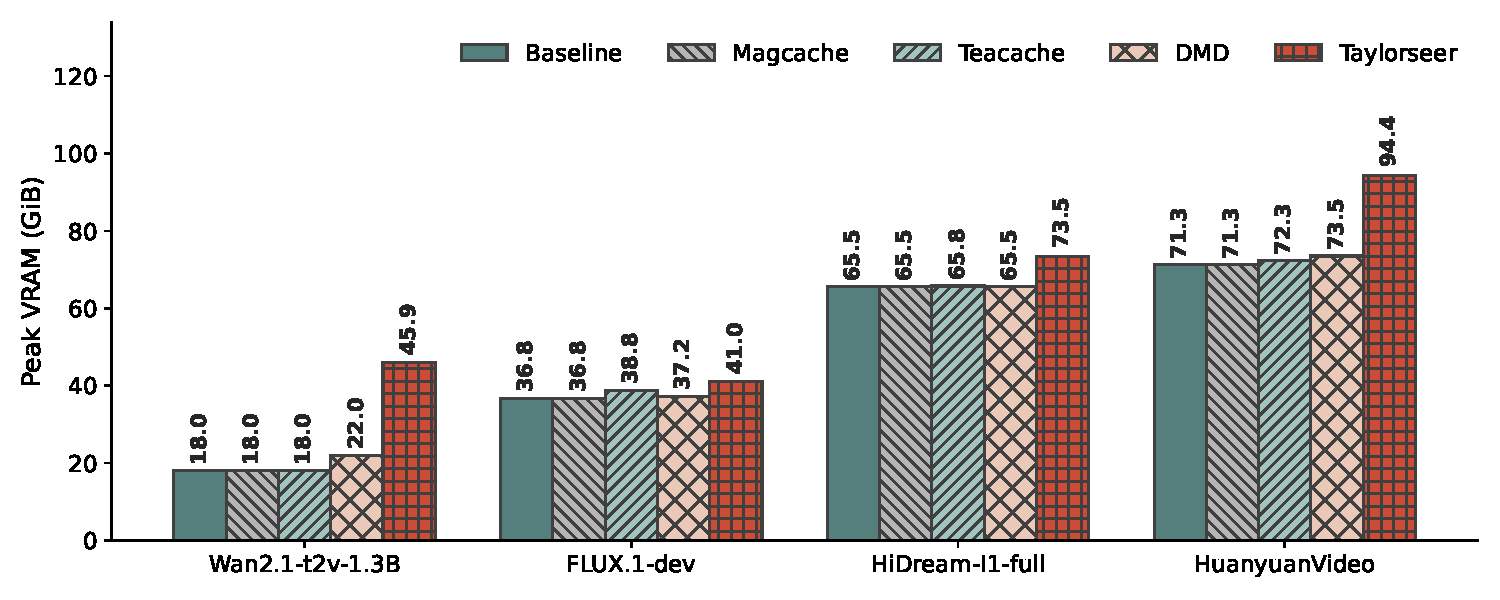
\includegraphics[width=\textwidth]{figures/vram_by_model_method.pdf}
    \caption{Peak VRAM footprint (GiB) across models and methods.}
    \label{fig:app:vram-by-model-method}
    \vspace{-10pt}
\end{figure}

\textbf{Discussion.}
\Cref{fig:app:vram-by-model-method}
demonstrates that TeaCache and MagCache track the baseline footprint closely,
while $D^3$-Cache incurs only minor overhead,
consistent with its design choice of caching only transformer output tensors.
In contrast,
TaylorSeer introduces substantial activation-cache overhead
that can dominate the memory budget on large video models,
restricting practical deployments.

\section{DMD Predictor Pseudocode}\label{app:dmd-pseudocode}

\begin{algorithm}[t]
\caption{DMD Prediction for Diffusion Outputs}
\label{alg:app:dmd-predict}
\begin{algorithmic}[1]
\Require History window $\mathcal{H}_k = \{\mathbf{y}_{k-m+1}, \ldots, \mathbf{y}_k\}$ with $\mathbf{y}_i \in \mathbb{R}^D$
\Require Mean timestep interval $\bar{\Delta t}$ and target interval $\Delta t_{k+1}$
\Ensure Predicted transformer output $\hat{\mathbf{y}}_{k+1} \in \mathbb{R}^D$
\State $\mathbf{X} \gets [\mathbf{y}_{k-m+1}, \ldots, \mathbf{y}_{k-1}]$, \quad
       $\mathbf{Y} \gets [\mathbf{y}_{k-m+2}, \ldots, \mathbf{y}_k]$
\State $r \gets \min(D, m-1)$
\State Compute compact SVD:
       $\mathbf{X} = \mathbf{U}_r \boldsymbol{\Sigma}_r \mathbf{V}_r^{\top}$
\State Lower-bound the diagonal entries of $\boldsymbol{\Sigma}_r$ by $\epsilon$
\State $\tilde{\mathbf{A}} \gets
       \mathbf{U}_r^{\top}\mathbf{Y}\mathbf{V}_r\boldsymbol{\Sigma}_r^{-1}$
\State Compute eigendecomposition:
       $\tilde{\mathbf{A}}\mathbf{W} = \mathbf{W}\boldsymbol{\Lambda}$
\State $\mathbf{\Phi} \gets
       \mathbf{Y}\mathbf{V}_r\boldsymbol{\Sigma}_r^{-1}\mathbf{W}$
\State $\mathbf{b} \gets \mathbf{\Phi}^{\dagger}\mathbf{y}_k$
\State $\boldsymbol{\omega} \gets \bar{\Delta t}^{-1}\log\!\left(\operatorname{diag}(\boldsymbol{\Lambda})\right)$
\State $\hat{\mathbf{y}}_{k+1} \gets
       \operatorname{Re}\!\left(\mathbf{\Phi}\left(\exp(\boldsymbol{\omega}\Delta t_{k+1}) \odot \mathbf{b}\right)\right)$
\State \Return $\hat{\mathbf{y}}_{k+1}$
\end{algorithmic}
\end{algorithm}
